\documentclass{article}
\usepackage{graphicx}
\usepackage{float}

\title{Analysis of Methodology for Motor Oil Time-Series Project}
\author{James Craven, Matthew Lindsey, Tina Lane}
\date{December 2024}

\begin{document}

\maketitle

\section{Business Understanding}
    \subsection{Objectives}
        The primary objective of this project is to experiment and develop practical experience in applying 
        data science techniques to a business problem, followed by the goal of forecasting motor oil sales 
        on a per-store basis. A secondary objective is to predict the future sales of specific products, 
        which will further support inventory planning, supply chain optimization, and resource allocation. \\
        \\
        To achieve these goals, the project will explore several related questions. For instance, how can 
        the dip in sales in 2020 be accounted for in the modelling process? Furthermore, how should unique 
        characteristics of the dataset, such as negative sales due to returns or high-value outliers, be 
        addressed to improve the reliability of the models? Addressing these questions ensures that the 
        project remains focused on delivering value while overcoming the challenges presented by the data. \\
        \\
        From a business perspective, the project will be judged on its capacity to deliver clear insights 
        into sales trends and anomalies. This translates to developing predictive models that effectively 
        handle missing values, anomalies, and other unique data characteristics from a data mining 
        perspective. Success criteria for data mining will include achieving forecasting models with 
        acceptable performance metrics to ensure predictive accuracy. Additionally, the project will compare 
        the performance of ARIMA and Prophet models, comparing their ability to forecast the sales data from 
        our dataset.
    \subsection{Analysis of Resources}
        The project is supported by several resources that enable its successful execution. The team 
        consists of three data science majors—Tina, Matthew, and James—who bring complementary skills in 
        data analysis, Python, and neural networks. \\
        \\
        Computing resources include access to college-provided facilities. Constraints while working on the 
        project may include limited time for experimentation with models. The project offers the team 
        academic and professional growth through the practical application of data science techniques.
    \subsection{Project Plan}
        This project was carried out over the course of the Fall 2024 semester at Winthrop
        University. The following plan was agreed upon at the beginning of the semester.
        Note that the weeks are relative to the semester, week 1 was focused on academic matters.
        Additionally, several weeks were missed due to severe weather and power outages.
        \begin{enumerate}
            \item \textbf{Weeks 2-3} - Data understanding phase
            \item \textbf{Weeks 4-5} - Data exploration, cleaning
            \item \textbf{Weeks 8-12} - Modelling phase
            \item \textbf{Weeks 13-14} - Evaluation
        \end{enumerate}


\section{Data Understanding}
    \subsection{Initial Data}
        The dataset for this project was provided to the authors of this report by a local
        data science company in Rock Hill, SC, called Delta Bravo. The dataset was an
        anonymized, unclean data set that had been brought upon by real-world clientele.
        The data set contains a time series representing semi-aggregate motor oil sales data.
    \subsection{Description}
        The data contained the following attributes:
        \begin{enumerate}
            \item \textbf{Invoice Date} - the date for which the total sales were recorded
            \item \textbf{Customer Code} - a code that uniquely identifies the customer. These codes
                were anonymized prior to receiving them in order to protect confidentiality
                of the original client.
            \item \textbf{Channel Text} - a label that represented the sales channel. This was almost
                entirely anonymized, and did not reveal any insights.
            \item \textbf{Blend} - The type of oil being sold. A categorical attribute that describing
                whether the oil is conventional or synthetic. This attribute was labelled internally
                as "conventional/synthetic"
            \item \textbf{Variety and Size} - details the oil type and packaging
            \item \textbf{Sale Value} - the target attribute, the total sales recorded for that row
        \end{enumerate}
    \subsection{Exploration}
        A notable feature of the dataset is the impact of the COVID-19 virus in the sales. A sharp
        decline can briefly be seen before slowly trending back up to pre-pandemic levels.
        Another key observation is the imbalance of both the spread of the location and the blend types.
        \begin{figure}[!h]
            \centering
            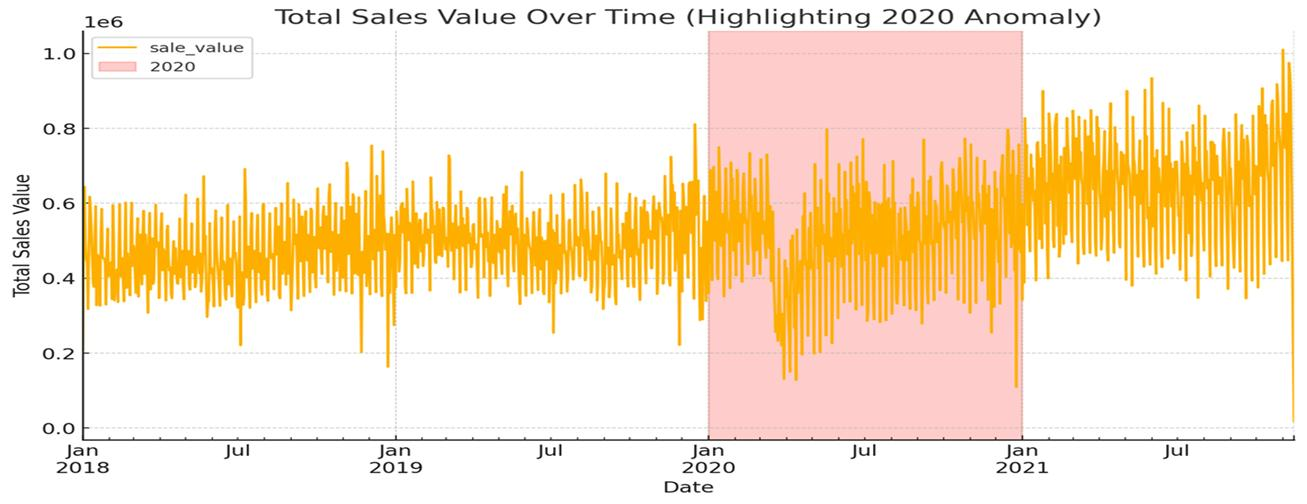
\includegraphics[width=0.9\linewidth]{assets/covid.jpg}
            \label{fig:covid}
        \end{figure}
        \begin{figure}[H]
            \centering
            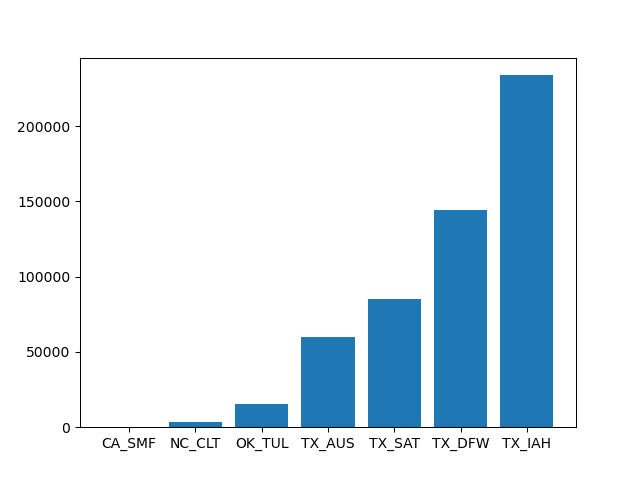
\includegraphics[width=0.8\linewidth]{assets/locations.png}
            \caption{number of data instances by location}
            \label{fig:locations}
        \end{figure}
        \begin{figure}[H]
            \centering
            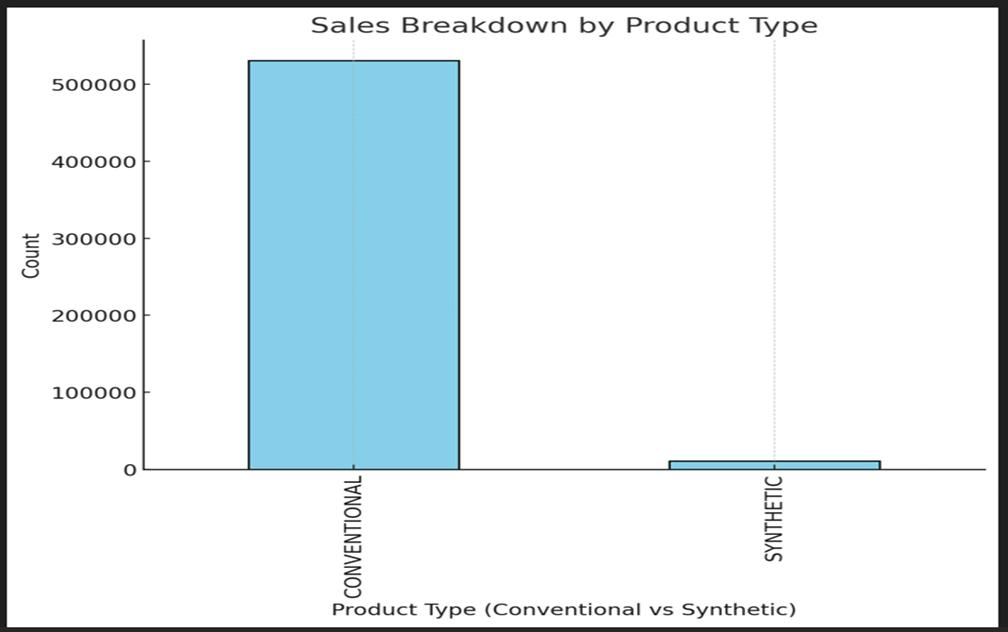
\includegraphics[width=0.6\linewidth]{assets/blend.jpg}
            \label{fig:blend}
        \end{figure}
        
        
\section{Data Preparation}
    \subsection{Data Selection}
        Using criteria derived from information inferred during the data understanding phase,
        various attributes were dropped for the sake of this project, leaving only the invoice
        date as an index of the data set, sale values, and the location of the store from which
        the sale was made. Customer status was immediately removed due to its singular
        cardinality, ruling it out as a potential source of signal for the model. The attributes
        customer code and channel text were likewise removed due to their lack of relevance in
        forecasting sale values. Size and variety were not immediately discarded, but were later
        dropped as they suffered from imbalanced spread and did not lend to the task at hand.
    \subsection{Data Cleaning \& Aggregation}
        Of the remaining attributes, two required additional cleaning: the invoice dates and the
        sale values. With respect to the invoice dates, there were some missing dates as well as
        duplicate values. It became clear that the dataset contained multiple sale values for the
        same days, and these values were aggregated on per-location basis. The missing dates had
        had their values using linear interpolation.
    \subsection{Data Integration}
        The resulting clean data was completely separated by location in order to preserve trend
        information related to local supply and demand as well as other regional factors.


\section{Modelling}
    \subsection{Modelling Technique}
        For this project, we utilized two time-series forecasting techniques, Prophet and ARIMA,
        to address our data mining problem. These two models were chosen, due to the educational
        nature of the project, to display the usage of explainable and unexplainable machine
        learning methods. \\
        \\
        Prophet was chosen as the unexplainable "black box" method as it uses neural networks to
        forecast based on the time-series it was trained on. It is considerably more flexible
        and performs well when given noisy data. ARIMA, on the other hand, is a widely known
        statistical approach to time-series data. Its reliance on autoregressive (AR), differencing
        (I), and moving average (MA) terms allows for precise modelling of linear patterns 
        in time-series data.
    \subsection{Test Design}
        To evaluate the two models' efficacy in forecasting the sales data, we performed a train-test
        split so that we can use the testing data to evaluate the models against actual data. By
        later testing these models, we can generate common time-series performance metrics like Root
        Mean Square Error (RMSE) and Akaike Information Criterion (AIC).
    \subsection{Building Models}
        By using AutoARIMA from the Python module "pmdarima" to automate parameter selection based on
        AIC optimization, we ensured optimal configurations of the model for daily and weekly data.
        The confidence intervals present in the ARIMA model provide great insights into ARIMA's 
        strengths and limitations.
        \begin{figure}[H]
            \centering
            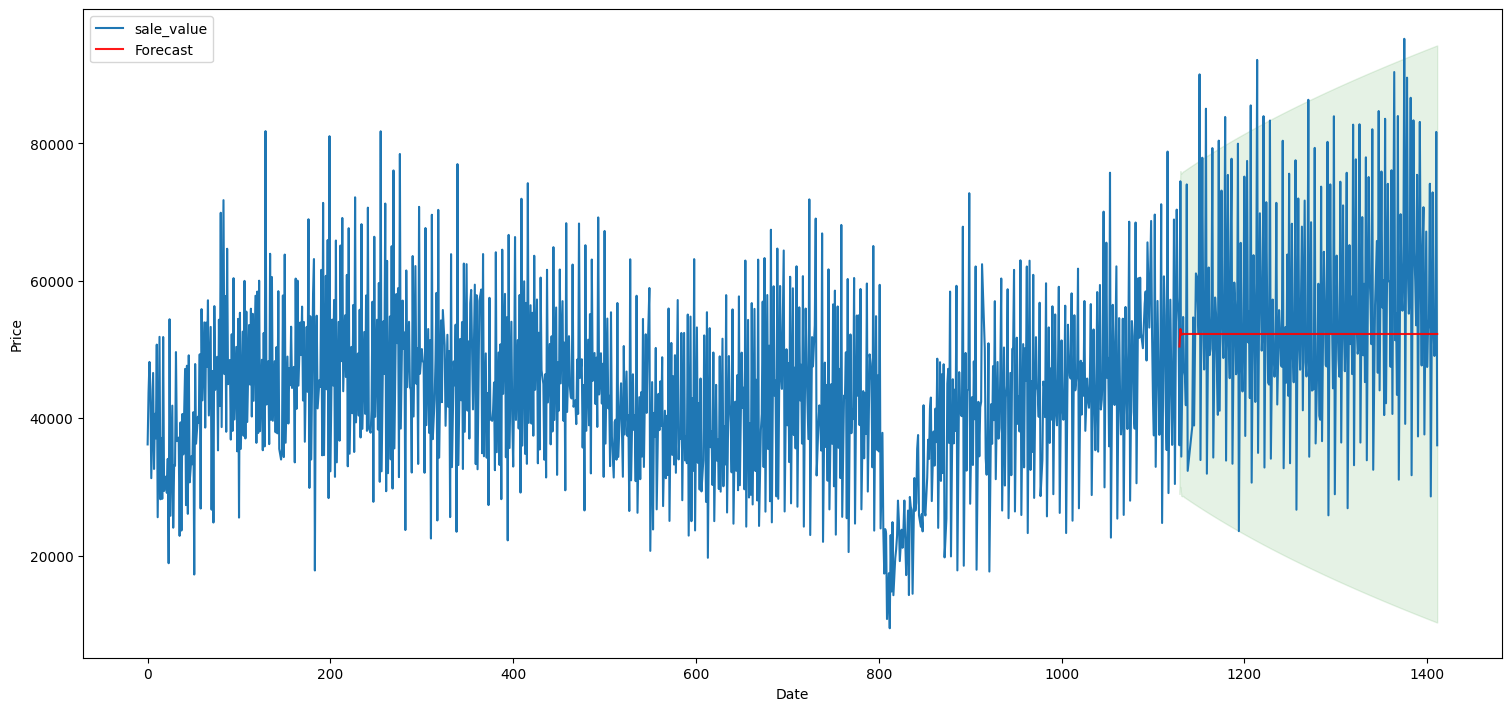
\includegraphics[width=0.85\linewidth]{assets/ARIMA-Daily.png}
            \caption{ARIMA forecast on TX AUS daily data}
            \label{fig:ARIMA-Daily}
        \end{figure}
        \begin{figure}[H]
            \centering
            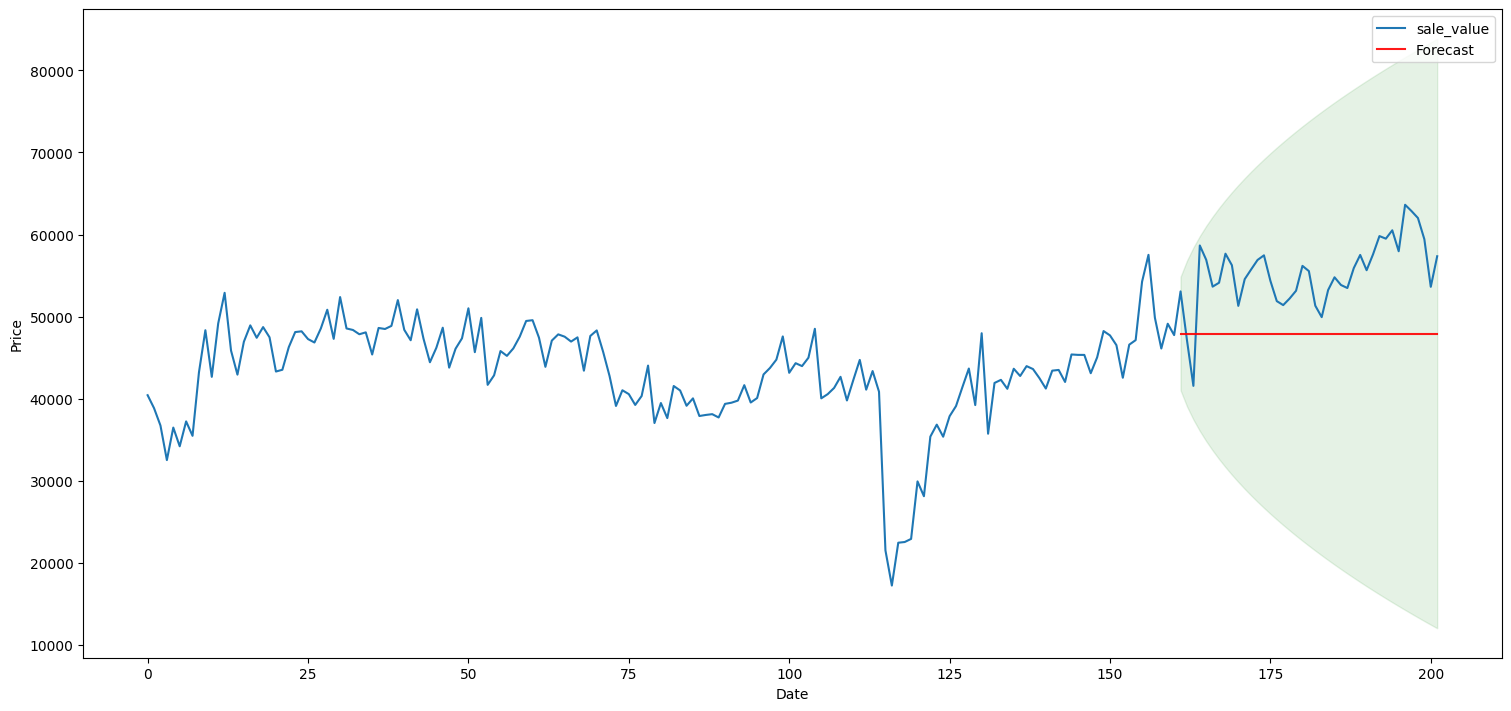
\includegraphics[width=0.85\linewidth]{assets/ARIMA-Weekly.png}
            \caption{ARIMA forecast on TX AUS weekly data}
            \label{fig:ARIMA-Weekly}
        \end{figure}
        For Prophet, we also trained models on both daily and weekly data. After training models 
        without accounting for the COVID-19 lockdowns, we tried to incorporate them as custom
        one-off holiday periods. Those models took into account the dip in sales in 2020.
        \begin{figure}[H]
            \centering
            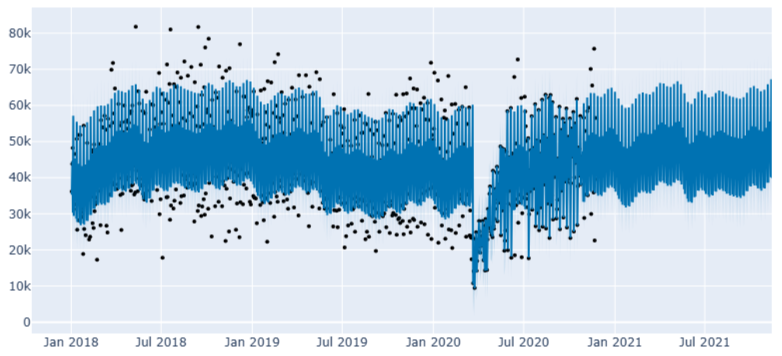
\includegraphics[width=0.85\linewidth]{assets/Prophet-Daily.png}
            \caption{Prophet forecast on TX AUS daily data}
            \label{fig:Prophet-Daily}
        \end{figure}
        \begin{figure}[H]
            \centering
            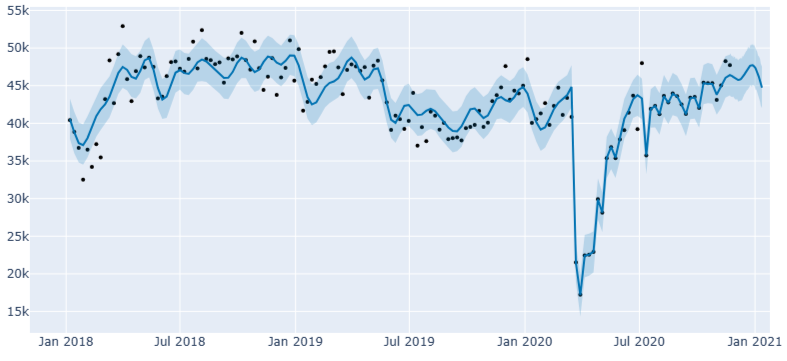
\includegraphics[width=0.85\linewidth]{assets/Prophet-Weekly.png}
            \caption{Prophet forecast on TX AUS weekly data}
            \label{fig:Prophet-Weekly}
        \end{figure}
    \subsection{Individual Assessment}
        Prophet models that incorporated lockdowns outperformed their counterparts without external 
        factors, demonstrating the importance of context-aware modelling. Weekly aggregation helped 
        reduce noise, thus had the lowest AIC and RMSE scores. \\
        \\
        ARIMA’s linear approach limited its ability to capture non-linear patterns, and generally 
        had higher AIC and RMSE scores. Again, Weekly aggregation produced better results by reducing
        noise from the daily data.


\section{Evaluation}
    \subsection{Assessment of Results}
        As stated previously, the metrics RMSE (Root Mean Squared Error) and AIC (Akaike Information 
        Criterion) were used to evaluate the models. RMSE measures predictive accuracy by capturing 
        the average magnitude of error, while AIC evaluates the model’s goodness of fit while 
        penalizing complexity. \\
        \\
        ARIMA models performed well in regions with consistent and stationary sales patterns. For 
        example, in TX DFW, ARIMA achieved an RMSE of 13,727 and an AIC of 34,327. However, 
        in more volatile regions like TX IAH, ARIMA’s RMSE increased to 18,734, and its AIC 
        rose to 45,219. \\
        \\
        Prophet consistently outperformed ARIMA across all regions, demonstrating superior 
        accuracy and adaptability. For instance, in TX DFW, Prophet achieved an RMSE of 11,429 
        (a 16.7 percent improvement over ARIMA) and an AIC of 33,218. Additionally, In regions like 
        CA SMF and TX SAT, where ARIMA performed relatively well, Prophet still demonstrated 
        improved results.
        \begin{figure}[H]
            \centering
            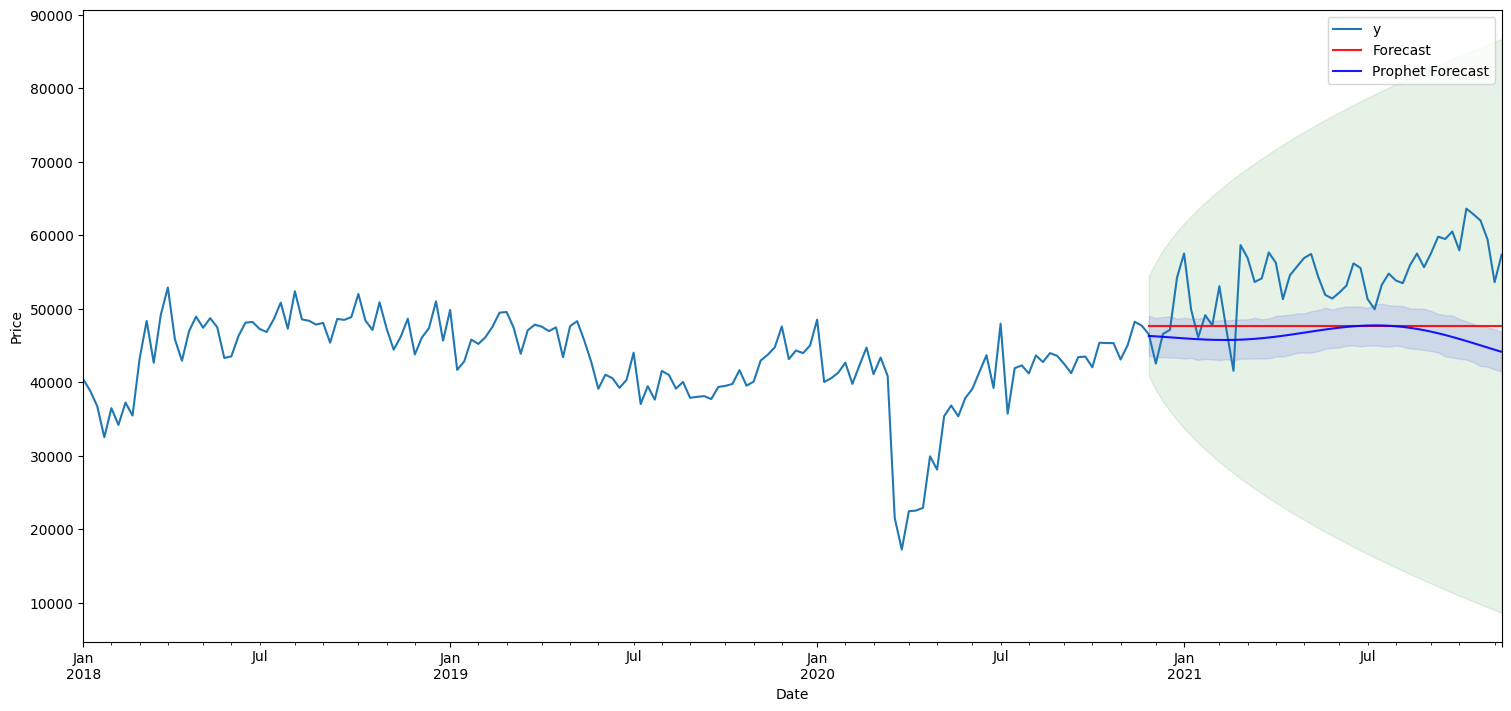
\includegraphics[width=0.85\linewidth]{assets/Model-Comparison.png}
            \caption{Comparing Prophet (Blue) and ARIMA (Red) with TX AUS forecast}
            \label{fig:Model-Comparison}
        \end{figure}
    \subsection{Finalized Models}
        The final models can be broken down into several different categories. Firstly, the type of 
        model, ARIMA or prophet. Secondly, the models were trained on different versions of the data.
        The data was aggregated either on a daily or weekly basis. Additionally the initial test train
        split was inadequate because the data had a sudden change in trend very close to the split date.
        To ensure model efficacy the models were also trained on just the original test data to see if it
        could accurately capture the new trend. Models were trained on all combinations of the aforementioned
        factors for at least one of the locations.
    \subsection{Future Action}
        Some features of the dataset, namely the variety of the oil, were not treated to the fullest
        extent that they could have been in this project. This is a weak point of the approach that
        was taken, and future efforts attempting to mitigate the imbalanced spread of the blend may
        take into account the effect of this and the varieties of oil to yield further insights
        about inventory and sales at a more granular level.
    \subsection{Conclusion}
        The ultimate purpose of this project was to acquaint the authors with time-series and different
        methodologies involved in the treatment of such. Thus it was decided that the project would
        act as a survey of both ARIMA and Neural Network based models, and as a comparison of the two.
        From the results of the modelling stage, we can conclude that both types of models tend to capture
        similar trends, but with varying levels of granularity and confidence. ARIMA casts a far wider net,
        so to speak, and as such values are far more likely to fall in its confidence interval. The prophet
        model, on the other hand, tends to be more confident in its prediction, however, if something unexpected
        happens, the actual data can fall far outside of its predicted bounds. Prophet is able to produce
        a forecast line that is more nuanced, though, and may be able to capture smaller, temporary noise
        slightly better as a result.

\end{document}